\documentclass[12pt,a4paper]{article}
\usepackage{amsmath}
\usepackage{amsfonts}
\usepackage{amssymb}
\usepackage{makeidx}
\usepackage{graphicx}
\usepackage[left=2cm,right=2cm,top=2cm,bottom=2cm]{geometry}
\usepackage{hyperref}
\usepackage{listings}
\title{Homework 2}
\author{Bert Peters --- s1147919}
\begin{document}
\maketitle

\section{Image retrieval}
\subsection{Screenshot}
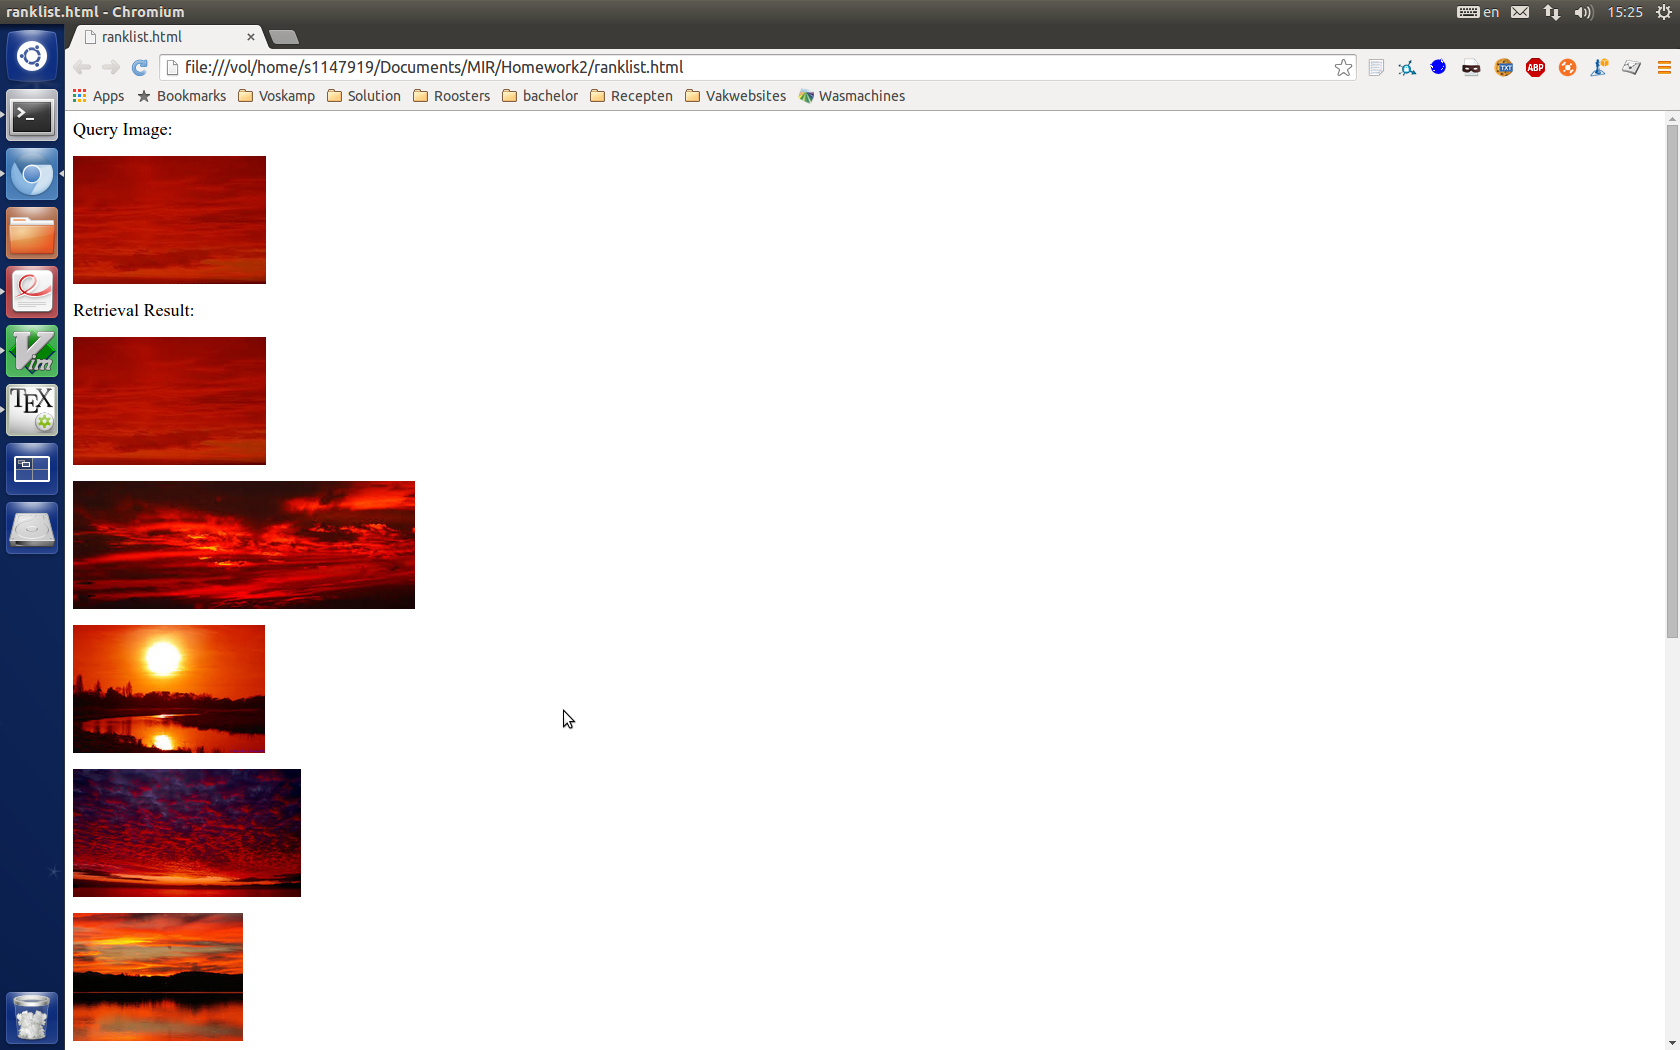
\includegraphics[scale=0.25]{screenshot}

\subsection{Experiments}

The program computes the average hue for every picture in the specified directory, and then ranks other pictures based on the similarity of that hue to the specified picture.

With the sample images, this works really well because they are really well defined red going to blue. This is not common to find in pictures. When you instead look at more natural pictures, the average hue is not that meaningful.

When you feed the algorithm pictures that do not have a well defined hue, the order is fairly random to a human. Sure, there still is an average hue but it says nothing about the similarity of the pictures.

\section{Downloading and parsing weblinks}

I have created a program that can scrape a web page for both image- and regular links. It then makes absolute links out of the results, and returns a string containing all links.

First, to write all CURL data to a string, we need to create a write callback function for CURL. This is the \texttt{WriteToMemory}. It needs to incrementally write the buffer, because CURL reports its data in several blocks. This is done using \texttt{realloc}.

The sample program provided already showed how to get the links from a stream. The only thing you still needed to do was adapt that to images. A regular link looks like an \texttt{<a>} tag with a \texttt{href} attribute. Image links are similar, being \texttt{<img>} tags with a \texttt{src} attribute.

To avoid repeating code, I have created a function \texttt{GetLinksByTag}, which gets a document as a character array, a base url, a tag name and an attribute name. This method is them called by \texttt{GetLinksFromWebPage} and \texttt{GetImageLinksFromWebPage} with the appropriate parameters.

The assignment specified that we had to print absolute links, rather than mixed links. In this exercise, we recognize three types of links:
\begin{description}
\item[Complete URLs] which start with a protocol (e.g. \texttt{http://}) and specify a domain etc. These can be used as is.

\item[Domain relative links] which start with a slash ('\texttt{/}') and should be resolved on the same domain. For example, on \url{http://liacs.leidenuniv.nl/} the link \\ \texttt{/organisatie/commissies/computercommissie/} should resolve to  \url{http://liacs.leidenuniv.nl/organisatie/commissies/computercommissie/}.

\item[Document relative links] which are resolved relative to the directory of the current document.\footnote{This can be overwritten using a \texttt{<base href="yourbase">} head directive. This tells the browser that document relative URLs should be resolved relative to that URL rather than the current document. In fact, \url{http://liacs.leidenuniv.nl/} uses this. This mechanism is also implemented.} For example, on \url{http://liacs.leidenuniv.nl/edu/}, the url \texttt{liacs/images/pijl.gif} should be expanded to \url{http://liacs.leidenuniv.nl/edu/liacs/images/pijl.gif}.
\end{description}
Creating absolute links is done in the \texttt{FormatLink} function, which takes a base url and a link and returns a new string, which must be freed afterwards.

Due to the way relativisation works, my program requires the protocol to be specified in the URL. Thus, you get a command like \texttt{./showlinks http://liacs.leidenuniv.nl}. A trailing slash is optional. The source code for \texttt{showlinks.c} is shown below.

Finally, I made some slight changes to \texttt{htmlstreamparser}, to make it compliant with C99. This was necessary because it specified an inline function in the header, which is not allowed.\footnote{Technically, it is allowed, but this causes linker warnings because the inlined function is not included in the object file.}

\subsection{Building the program}

The program can be built using GNU make. It has been tested on GCC 5.3 and 4.6. Other versions will probably work as well.

\section*{Code listing}
\lstinputlisting[language=c, frame=L, label=showlinks.c, tabsize=2, breaklines, numbers=left]{websearch/showlinks.c}

\end{document}